\chapter{Low-Level Design (LLD)}

\section{LLD Overview}
The Low-Level Design (LLD) provides an in-depth, class-level, and schema-level specification of Lucid's software components, data structures, algorithm implementations, and sequence flows. It translates the high-level architecture into precise technical abstractions implemented across the Next.js frontend, FastAPI backend, LangGraph agent workflows, and quantitative optimization engines.

\section{Frontend Architecture and Component Hierarchy}
The client application is built with \textbf{Next.js 16.4.2} utilizing the React 19 App Router architecture (\texttt{frontend/src/app/}). State management leverages React hooks (\texttt{useState}, \texttt{useEffect}, \texttt{useCallback}) alongside local storage caching for authenticated session tokens.

\subsection{Component Structure and Responsibilities}
The presentation tier is structured into modular, decoupled React components located in \texttt{frontend/src/components/}:
\begin{itemize}
    \item \textbf{\texttt{Navbar.tsx} \& \texttt{Footer.tsx}}: Navigation header managing global auth state, active user profile, Demat connection status, and responsive layout toggles.
    \item \textbf{\texttt{LandingPage.tsx}}: Marketing hero section, feature highlights, and interactive entry points for new and returning investors.
    \item \textbf{\texttt{AuthView.tsx} \& \texttt{ProfileAuthModal.tsx}}: Authentication dialogs managing email/password registration, login, JWT token persistence, and input validation.
    \item \textbf{\texttt{OnboardingWizard.tsx} \& \texttt{RiskQuestionnaireView.tsx}}: Five-step wizard presenting SEBI suitability questions, computing real-time risk scores, and persisting assessment results.
    \item \textbf{\texttt{PortfolioGenerator.tsx}}: Interactive portfolio configuration panel allowing users to specify investment capital, select or define financial goals, and set sector preferences or exclusions.
    \item \textbf{\texttt{HoldingsView.tsx} \& \texttt{AllocationVisualizer.tsx}}: Portfolio display interface rendering holding tables, whole-share lot quantities, average purchase prices, live NAV, and interactive sector/asset breakdown charts.
    \item \textbf{\texttt{StockWhyModal.tsx} \& \texttt{ExplainabilityView.tsx}}: Fiduciary explainability modals rendering dual-level justifications (retail narrative and quantitative econometric factor scores).
    \item \textbf{\texttt{DiagnosisView.tsx} \& \texttt{DiagnosisCopilotModal.tsx}}: Drag-and-drop PDF CAS statement uploader, holdings extraction parser, and AI-assisted Demat health diagnostic interface.
    \item \textbf{\texttt{RebalancePreviewModal.tsx}}: Interactive modal displaying proposed BUY/SELL share orders, net cash changes, and statutory transaction cost breakdowns.
    \item \textbf{\texttt{BenchmarksView.tsx} \& \texttt{StressScenariosView.tsx}}: Comparative performance analytics comparing Lucid against Equal-Weight (1/N) and Nifty 50 benchmarks, including stress testing under historical market shocks.
    \item \textbf{\texttt{ConversationalAssistant.tsx}}: Natural language chat interface enabling investors to query portfolio decisions and explore stock rationale interactively.
    \item \textbf{\texttt{NotificationsPanel.tsx}}: Real-time notification drawer displaying drift alerts, rebalance recommendations, and system events.
\end{itemize}

\subsection{Type-Safe Client API Layer (\texttt{frontend/src/lib/api.ts})}
All network communication with the backend is abstracted through a type-safe API module. It handles:
\begin{itemize}
    \item Dynamic base URL resolution (\texttt{http://localhost:8000}).
    \item Automatic injection of \texttt{Authorization: Bearer <token>} headers.
    \item Unified response parsing and error handling, mapping HTTP status codes (400, 401, 403, 404, 422, 429, 500) into structured UI alerts.
\end{itemize}

\section{Backend Architecture and API Subsystem}
The backend is structured as a modular, layered FastAPI application under \texttt{backend/}:

\begin{verbatim}
backend/
|-- api/
|   `-- v1/              # Versioned API routes (82 endpoints)
|       |-- auth.py      # Authentication, login, registration, JWT
|       |-- users.py     # Profile management, preferences
|       |-- risk.py      # Suitability questionnaire & scoring
|       |-- goals.py     # Financial goal CRUD & progress tracking
|       |-- market_data.py # Quotes, historical prices, regime, universe
|       |-- portfolios.py # Generation requests, versioning, stock-why
|       |-- diagnosis.py # Demat CAS PDF parsing & health diagnosis
|       |-- monitoring.py # Portfolio valuation & drift tracking
|       |-- rebalancing.py # Rebalancing strategy & order previews
|       |-- notifications.py # Real-time alerts
|       `-- broker.py    # Broker simulation & order execution
|-- models/              # SQLAlchemy 2.0 ORM domain models (62 tables)
|-- schemas/             # Pydantic v2 request & response validation schemas
|-- services/            # Business logic and external service orchestrators
|-- portfolio_engine/    # Quantitative optimization, rounding, transaction costs
|-- agents/              # LangGraph multi-agent StateGraph workflow
|-- database/            # Engine configuration, sessionmaker, get_db dependency
|-- middleware/          # Rate limiting, security headers, CORS
|-- alembic/             # Database migration revisions
`-- config.py            # Centralized settings (pydantic-settings)
\end{verbatim}

\subsection{Dependency Injection and Session Management}
FastAPI's dependency injection system (\texttt{Depends}) manages transactional database sessions:
\begin{equation}
\text{get\_db}() \to \text{Generator}[\text{Session}, \text{None}, \text{None}]
\end{equation}
The \texttt{get\_db} dependency yields a thread-local SQLAlchemy \texttt{SessionLocal} bound to PostgreSQL, ensuring that database connections are returned to the connection pool (\texttt{pool\_size=10, max\_overflow=20}) immediately upon request completion.

\section{Agent-Level Design: 13-Node LangGraph StateGraph}
The multi-agent workflow is implemented in \texttt{backend/agents/graph.py} and \texttt{backend/agents/state.py} using \textbf{LangGraph 0.4}. The state across the entire execution graph is governed by a unified TypedDict:

\begin{verbatim}
class AgentState(TypedDict):
    request_id: str
    user_id: str
    risk_category: str          # conservative, moderate, aggressive
    investment_amount: float
    goal_type: Optional[str]
    time_horizon_years: Optional[int]
    macro_regime: Dict[str, Any]
    market_volatility: Dict[str, Any]
    candidate_universe: List[Dict[str, Any]]
    fundamental_scores: Dict[str, float]
    sentiment_scores: Dict[str, float]
    critic_feedback: List[str]
    optimized_allocations: List[Dict[str, Any]]
    fiduciary_explanations: Dict[str, str]
    validation_status: bool
    error_messages: List[str]
\end{verbatim}

\subsection{Agent Nodes and Execution Topology}
The 13 nodes of the StateGraph execute in structured sequence with conditional validation edges:
\begin{enumerate}
    \item \textbf{Input Validation Node}: Validates investor capital ($\ge \text{Rs.~}5,000$), risk category, and time horizon.
    \item \textbf{Macro Analyst Node}: Analyzes RBI repo rate trends, inflation metrics, and GDP forecasts.
    \item \textbf{Market Regime Node}: Evaluates India VIX volatility tiers and Nifty 50 50-DMA/200-DMA technical trends.
    \item \textbf{Universe Ingestion Node}: Queries PostgreSQL for active listed equities matching liquidity thresholds.
    \item \textbf{Fundamental Analyst Node}: Filters candidates against balance sheet criteria (ROE $\ge 15\%$, Debt/Equity $\le 1.5$, positive operating cash flows).
    \item \textbf{Sentiment \& News Node}: Assesses ingested corporate news sentiment and corporate governance filings.
    \item \textbf{Valuation Screening Node}: Evaluates relative P/E, P/B, and historical EV/EBITDA ratios against industry benchmarks.
    \item \textbf{Candidate Ranking Node}: Combines fundamental, sentiment, and valuation scores into an aggregate conviction score.
    \item \textbf{Adversarial Critic Node}: Challenges top-ranked candidates, searching for unaddressed regulatory risks, sector concentration traps, or cyclical headwinds.
    \item \textbf{Quantitative SLSQP Solver Node}: Formulates and executes SciPy constrained mean-variance optimization.
    \item \textbf{Integer Lot Sizing Node}: Translates percentage weights into whole shares and computes residual cash.
    \item \textbf{Deterministic Constraint Validator Node}: Validates that no single stock exceeds 25\% and no sector exceeds 40\%. If violated, routes back to SLSQP with tightened bounds.
    \item \textbf{Dual-Level Explainability Node}: Generates user-facing retail narratives and structured econometric factor scorecards.
\end{enumerate}

\section{Quantitative Optimization and Lot Sizing Engine}
Located in \texttt{backend/portfolio\_engine/}, the quantitative engine implements:
\begin{itemize}
    \item \textbf{Optimizer (\texttt{optimizer.py})}: Configures the SLSQP solver (\texttt{scipy.optimize.minimize}), setting objective functions to minimize negative Sharpe ratio (or minimize portfolio variance for conservative profiles).
    \item \textbf{Integer Lot Rounder (\texttt{integer\_rounding.py})}: Executes whole-share floor rounding:
    \begin{equation}
    q_i = \left\lfloor \frac{C \cdot w_i^*}{P_i} \right\rfloor, \quad \text{Residual Cash} = C - \sum_{i=1}^{K} q_i P_i
    \end{equation}
    where $C$ is total capital, $w_i^*$ is optimal continuous weight, and $P_i$ is current stock price. A secondary heuristic pass allocates residual cash to the highest-conviction holdings whose unit prices fit within the remaining cash balance without breaching the 25\% single-stock ceiling.
    \item \textbf{Transaction Cost Engine (\texttt{transaction\_costs.py})}: Calculates all Indian statutory costs (STT 0.1\%, Exchange charges 0.00325\%, SEBI turnover fee 0.0001\%, Stamp duty 0.015\%, and GST 18\% on brokerage and exchange fees).
\end{itemize}

\section{Monitoring Scheduler and Distributed Locking}
Located in \texttt{backend/services/monitoring\_scheduler.py}, the unattended background monitoring service runs on a dedicated background thread with an asynchronous execution loop (\texttt{interval\_seconds=300}). 

To prevent concurrent execution across multi-worker deployments (e.g., multiple Uvicorn instances), the scheduler implements \textbf{PostgreSQL Session-Level Advisory Locking}:
\begin{equation}
\text{SELECT pg\_try\_advisory\_lock}(847291)
\end{equation}
Only the worker instance that acquires the 64-bit lock proceeds with portfolio valuation and drift auditing; secondary workers log an informative skip message and release the cycle.

\section{Sequence Flow Diagrams}
Figures~\ref{fig:seq_auth} through \ref{fig:seq_diag} illustrate the low-level sequence interactions for primary system operations.

\begin{figure}[H]
    \centering
    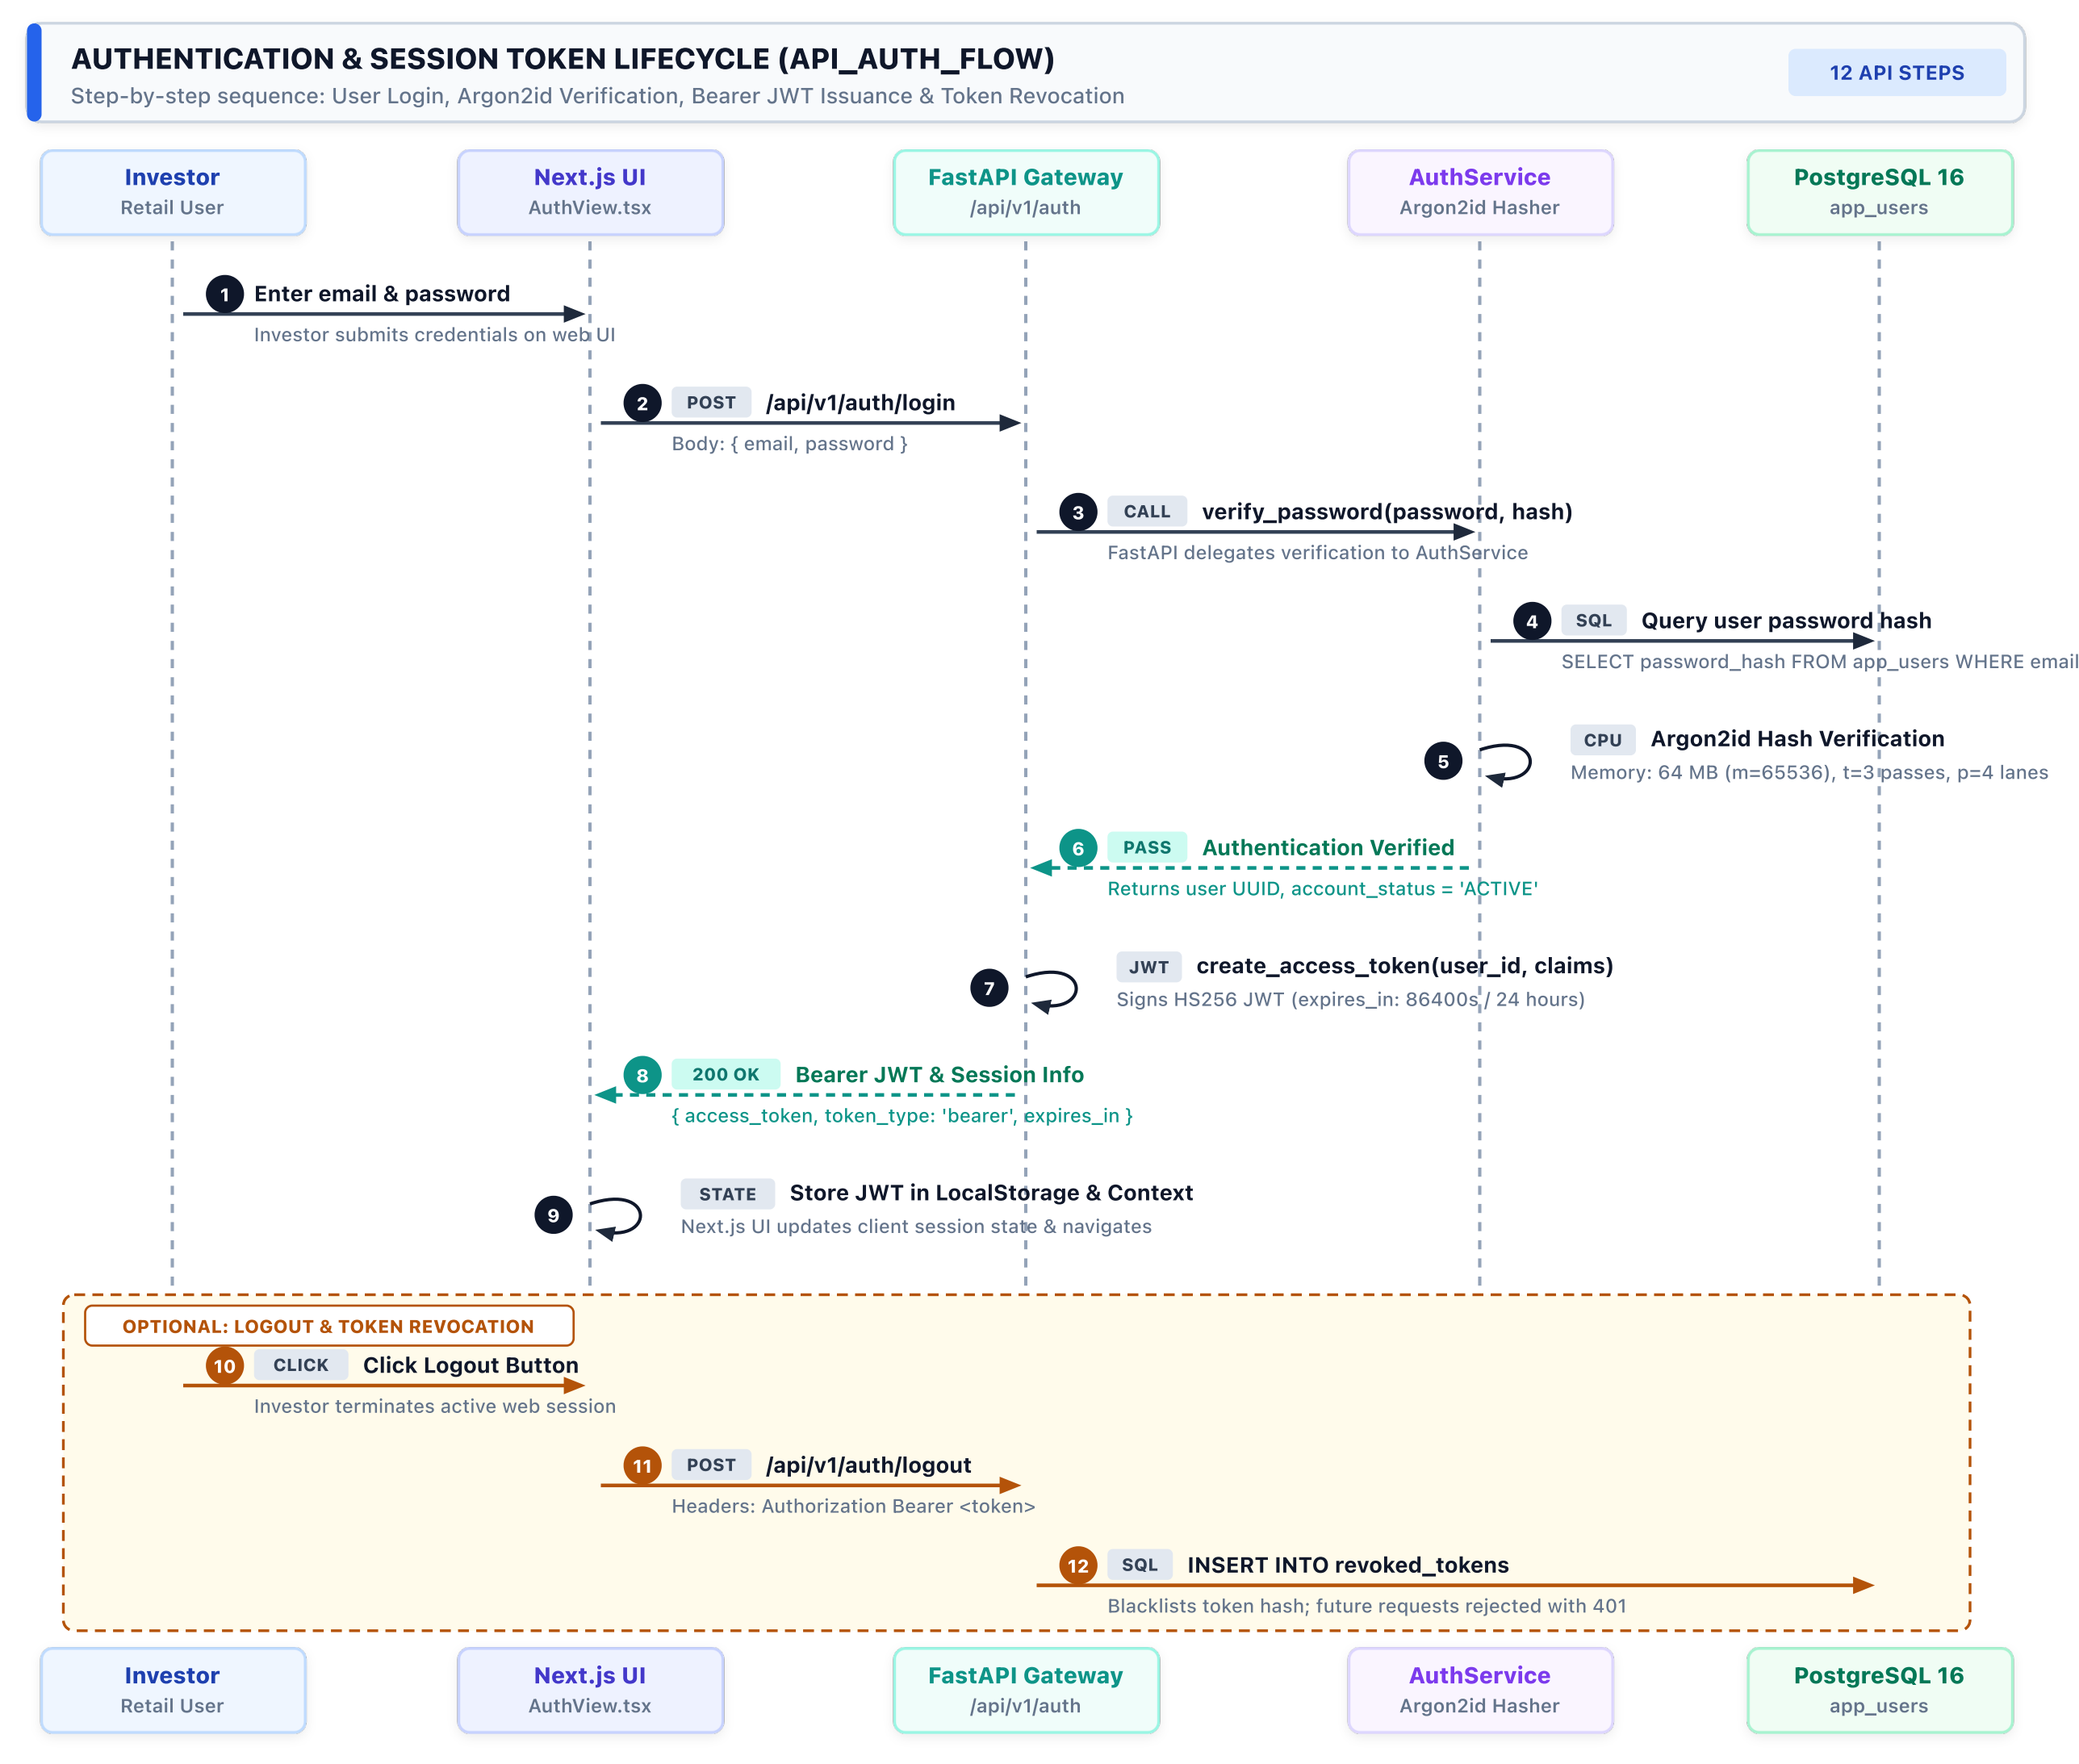
\includegraphics[width=0.9\textwidth]{API_AUTH_FLOW.png}
    \caption{Low-Level Sequence Flow: Investor Authentication and JWT Token Lifecycle}
    \label{fig:seq_auth}
\end{figure}

\begin{figure}[H]
    \centering
    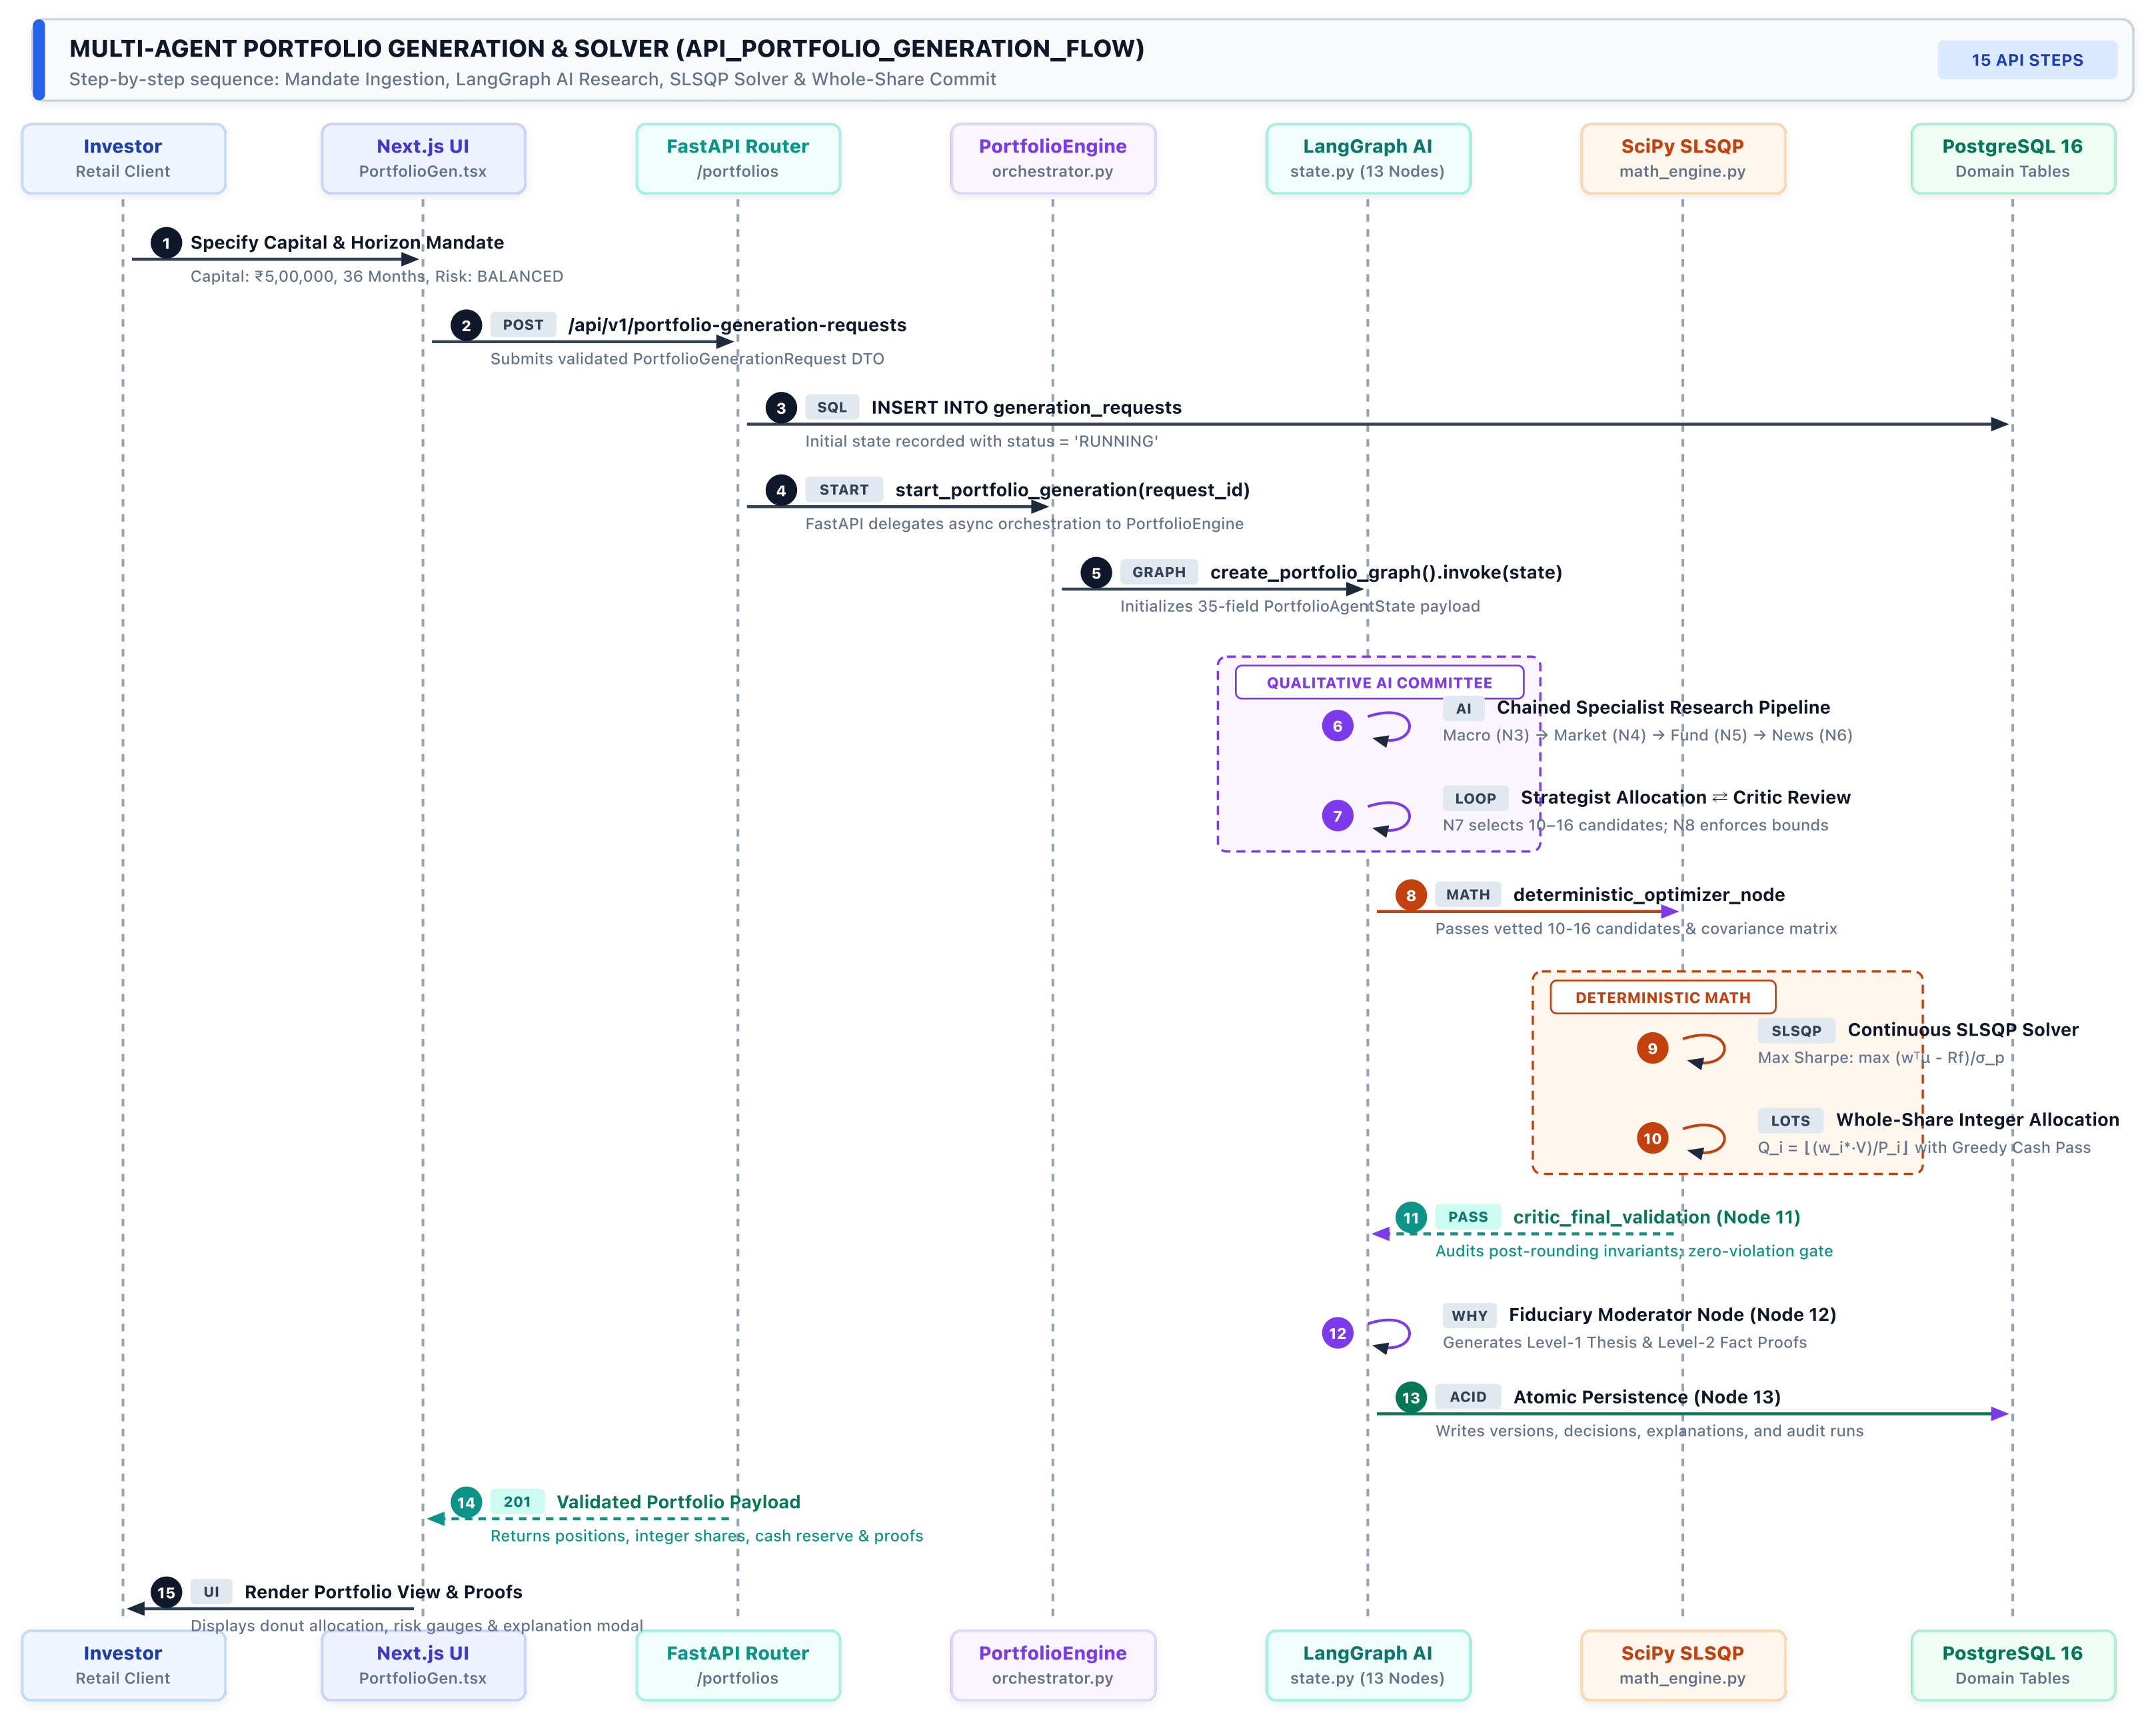
\includegraphics[width=0.95\textwidth]{API_PORTFOLIO_GENERATION_FLOW.png}
    \caption{Low-Level Sequence Flow: Goal-Driven Portfolio Generation and SLSQP Optimization}
    \label{fig:seq_generation}
\end{figure}

\begin{figure}[H]
    \centering
    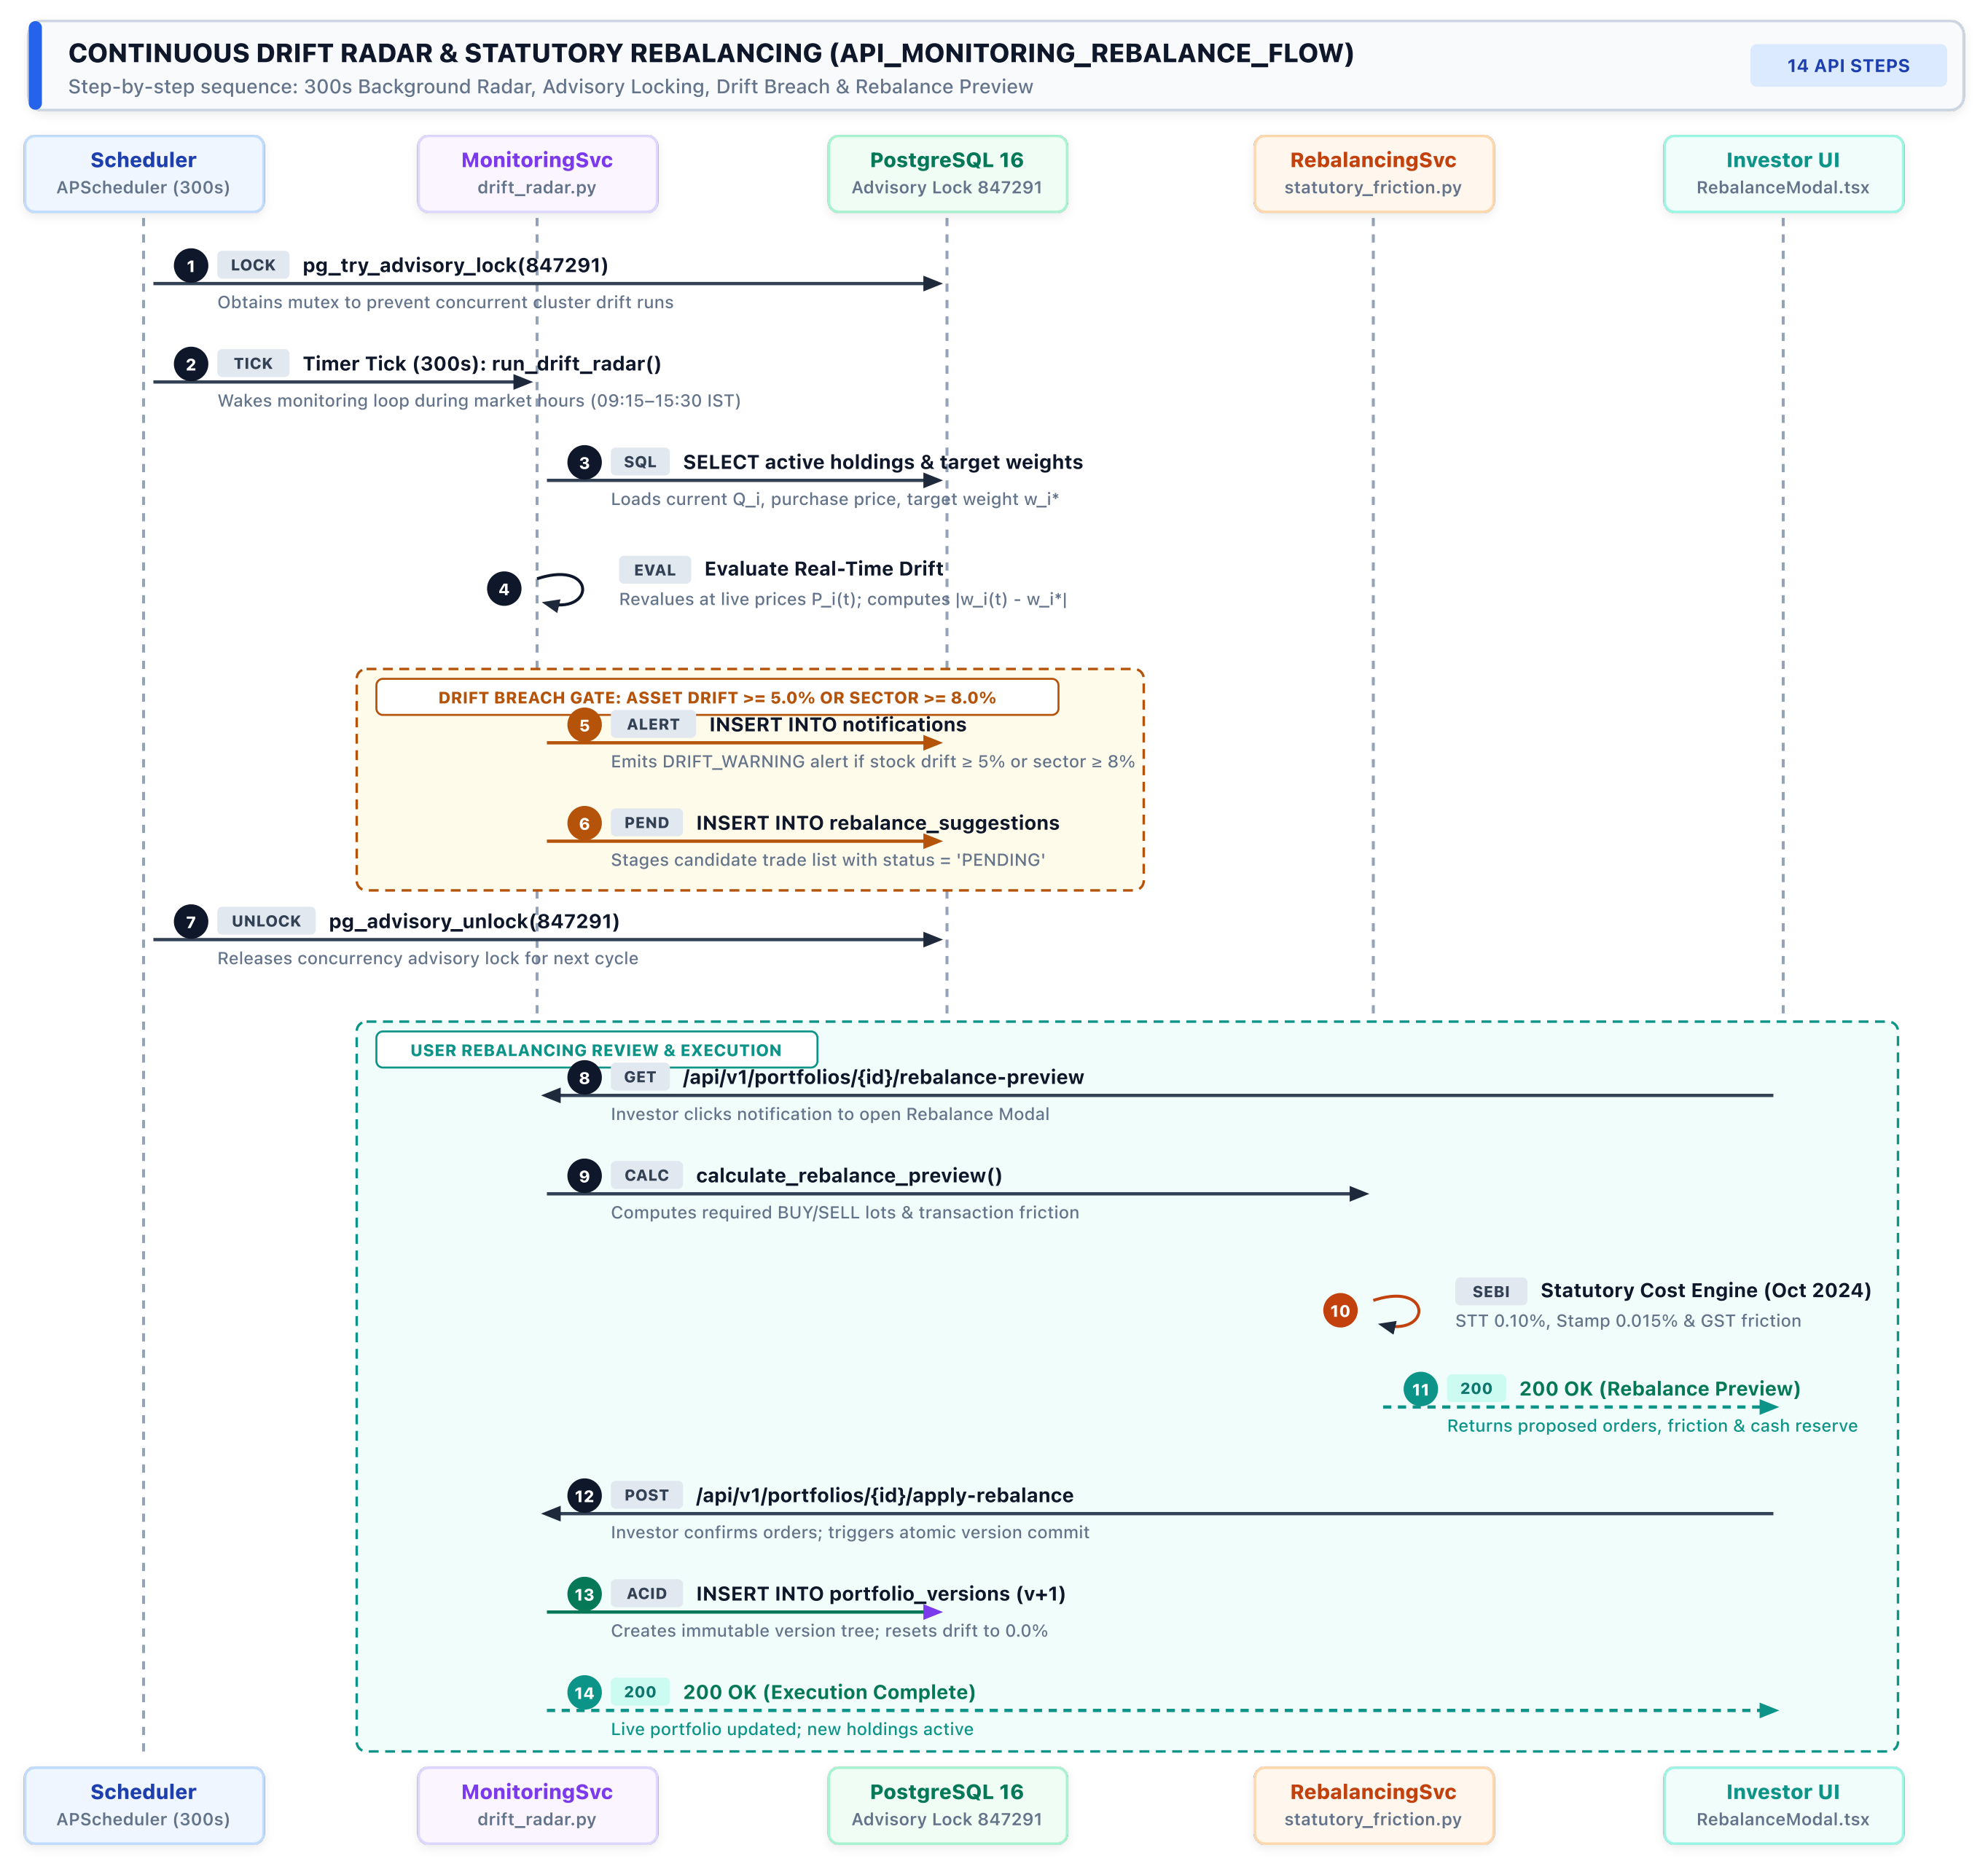
\includegraphics[width=0.95\textwidth]{API_MONITORING_REBALANCE_FLOW.png}
    \caption{Low-Level Sequence Flow: 5-Minute Drift Radar and Friction-Aware Rebalancing Preview}
    \label{fig:seq_monitoring}
\end{figure}

\begin{figure}[H]
    \centering
    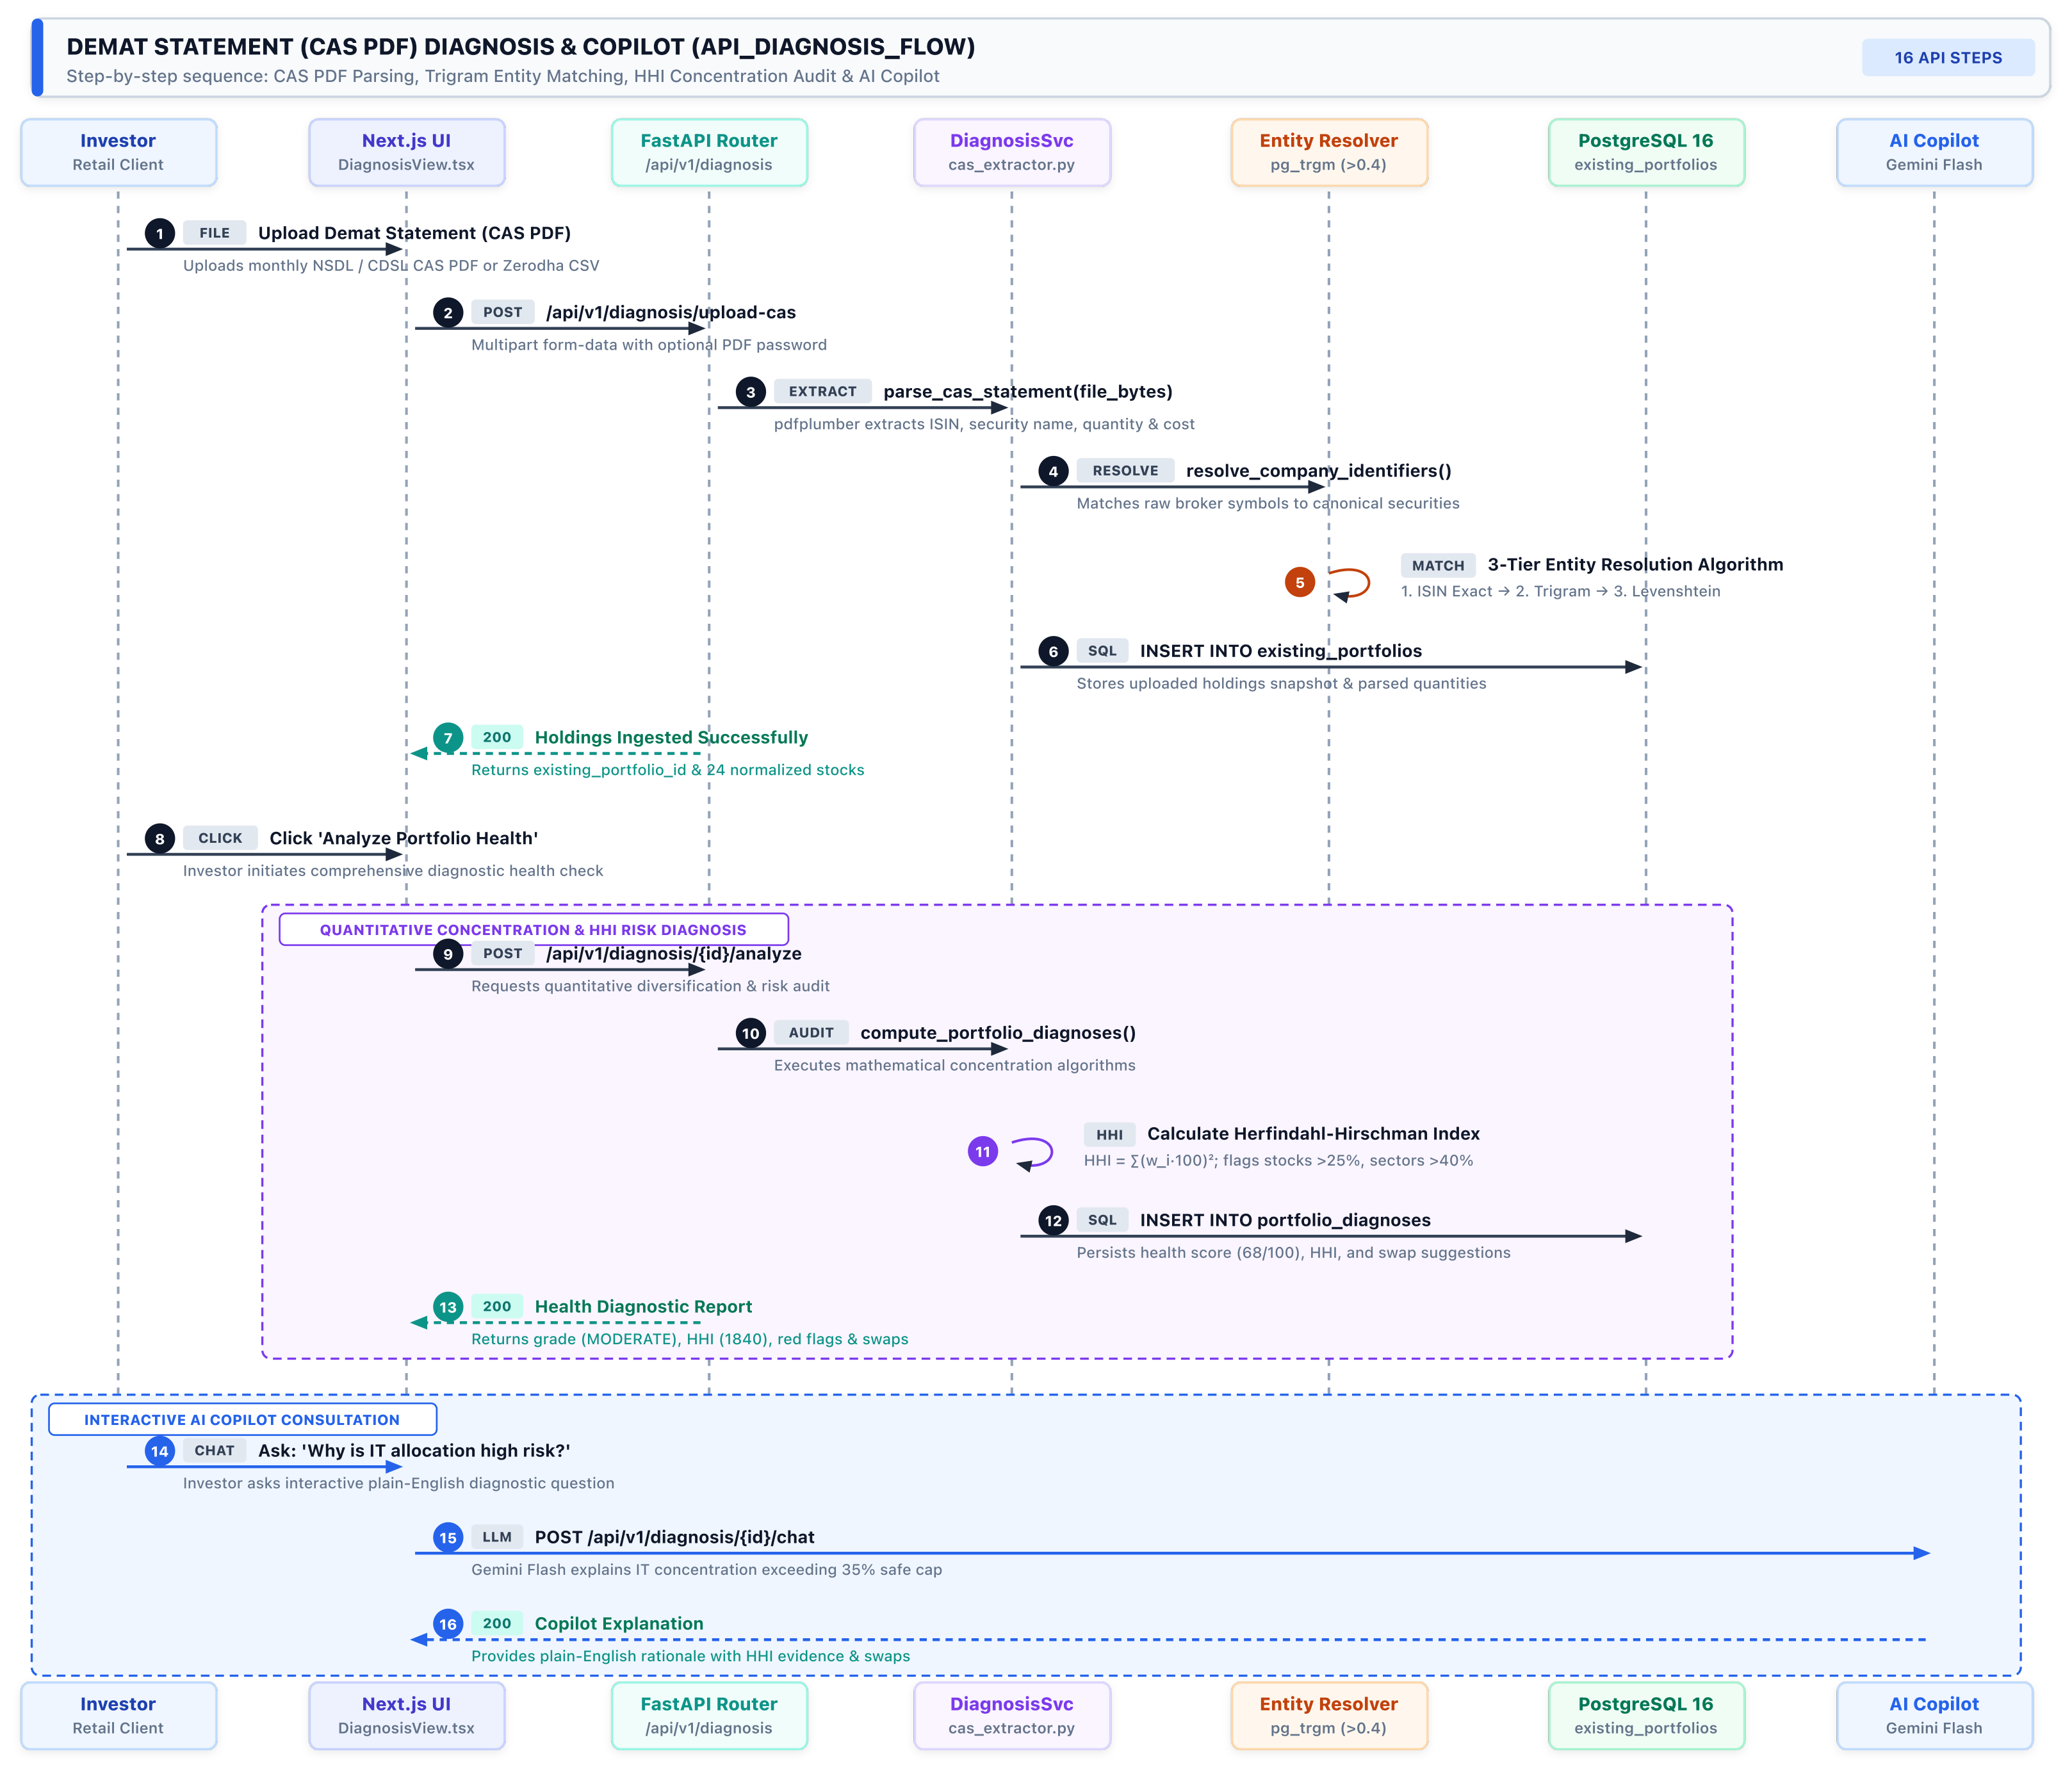
\includegraphics[width=0.95\textwidth]{API_DIAGNOSIS_FLOW.png}
    \caption{Low-Level Sequence Flow: Demat CAS PDF Statement Ingestion and Health Diagnosis}
    \label{fig:seq_diag}
\end{figure}
